For at kunne imødekomme et bredt spektrum af lidelser samt et bredt udvalg af forskellige, Android baserede, smartphones kræves en modulær arkitektur hvori moduler kan fjernes, tilføjes og ændres uafhængigt af det overordnede system.

Moduler inddeles i tre konceptuelle lag: \textit{sensor}-, \textit{analyse}- og \textit{visnings}moduler.
Denne inddeling vil tillade adskilt udvikling af enkelte moduler uanset hvilket lag de tilhører.
Ved at kombinere de forskellige moduler på tværs af lagene, opnås et fungerende system.

Eksempelvis vil et accelerometer \textit{sensor}modul kunne anvendes af et søvn \textit{analyse}modul der viser resultatet i et graf \textit{visnings}modul.
Skulle man her ønske en anden fortolkning af accelerometerets data kan et andet analysemodul anvendes.
Sammensætningen af analyse- og visningsmoduler sker ved en beskrivelse af deres grænseflade.
Moduler med fælles grænseflade vil kunne kombineres.
Det vil sige at der kan anvendes flere forskellige visningsmoduler til det samme analysemodul, givet at de er kompatible.
Tilsvarende kan det samme visningsmoduler anvendes til flere forskellige analysemoduler.
\textbf{Det har ikke været muligt at finde et umiddelbart arkitektur-mønster for dette.}
\stefan{vi bør nok udvide dette, det virker lidt tyndt at skrive}
\ivan{Enig. Check lige
	Gamma et al om
	I har overset noget.
	Samme om Fowler.
	HVIS der ikke
	findes mønstre, så
	tag nogle, der
	næsten gør, og
	forklar hvorfor de
	ikke kan bruges
	alligevel.}

\section*{Opbygning}
Den overordnede arkitektur er opbygget af fire komponenter: \textit{manager}, \textit{moduler}, \textit{DB access} og \textit{DB}.\ivan{evt. to ord om hver komponents formål}
En skitse af arkitekturen kan ses på \cref{arkitektur_udkast_1}.
\begin{figure}[h]
	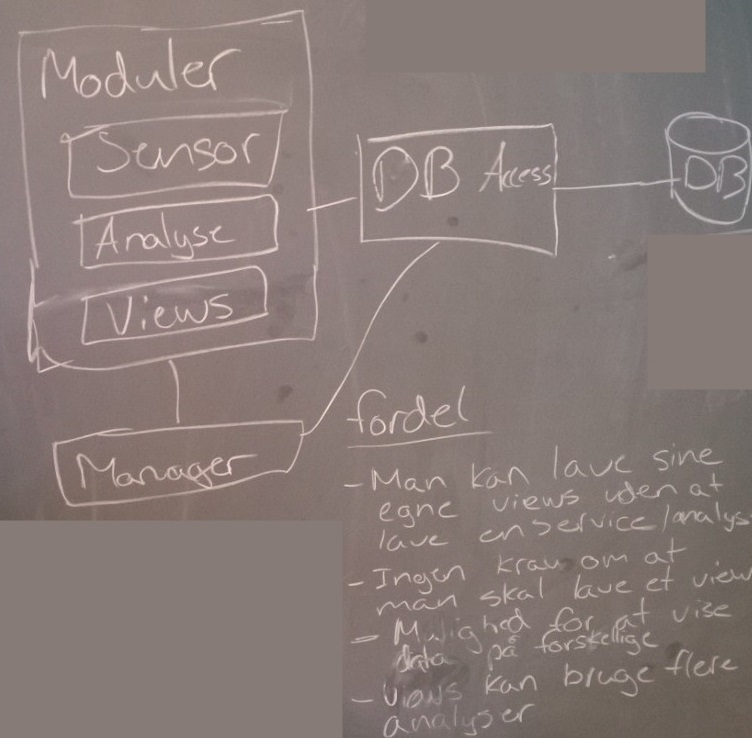
\includegraphics[width=\textwidth]{architecture_draft}
	\caption{Første udkast til arkitektur.}
  \label{arkitektur_udkast_1}
\end{figure}
Som nævnt herover er styrken ved denne arkitektur, den modulære opbygning af sensorer, analyser og visninger.
Disse lag er derfor alle indholdt i den overordnede komponent \textit{moduler}.
Derudover eksisterer et system, bestående af de resterende tre komponenter, der anvender de moduler der er installeret på den enkelte telefon. \ivan{kompakt og lidt klodset formulering}
Systemet er altså opbygget uden \ivan{evt. to ord om hver komponents formål} til de enkelte moduler, hvilket igen tillader udviklingen af moduler sideløbende med det overordnede system.
\ivan{Information hiding? Lidt tyndt her}

Herunder gives en kort beskrivelse af hver af de fire komponenter.
Komponenterne beskrives i rækkefølge af deres indbyrdes afhængighed, således at forståelsen af hver komponent kun afhænger af det læste.

\ivan{Måske var det en ide at bruge en skabelon for gennemgangen af komponenterne f.eks. (1) Formål - (2)design, og - (3) Perspektiv for fremtidig udvikling - På den måde kunne I understrege generaliteten og fremtidsikringen i jeres design}
\subsection*{DB}
Denne komponent administrerer data for systemets forskellige moduler.
Data opbevares i en række tabeller i et relationelt database system.
Hvert modul har mulighed for at definere egne tabeller, der alle gemmes i \textit{DB} komponenten.

Til dette projekt er valgt en SQLite database da denne er standard i Android.

\subsection*{DB Access}
Denne komponent styrer adgangen til \textit{DB} komponenten så det sker på en ensrettet måde.
Derudover skal \textit{DB Access} også sørge at et komponent kun kan skrive til sine egne tabeller, men have mulighed for at læse fra de tabeller som den er afhængig af.
Dette er dog ikke muligt da \textit{DB Access} bruger en \textit{ContentProvider}, men her er det ikke muligt at se hvad for en anden applikation der tilgår \textit{DB Access}, hvilket gør at denne begrænsning ikke er mulig. \ivan{Klodet og redundant sprog}

Systemet anvender udelukkende en database placeret på selve mobiltelefonen og er dermed begrænset af de muligheder der er for lagring på den enkelte enhed.
I en fremtidig udvidelse af systemet kunne \textit{DB Access} komponenten tilgå et ekstern lager hvor dele af det administrerede data kan gemmes.
Denne abstraktion forventes at kunne påføres \textit{DB Access} uden at kræve ændringer i de resterende komponenter.

Muligheden for en sådan udvidelse af systemet er ikke undersøgt og der kan derfor naturligt være komplikationer herved, ligesom udvidelsen ikke med sikkerhed kan laves uden påvirkning af de resterende komponenter.

\subsection*{Moduler}
Denne komponent består af de tre forskellige modul-lag.
Til hvert enkelt modul hører en modulbeskrivelse (se \cref{modul_definition}) der beskriver modulets afhængigheder af andre moduler samt hvordan det skal administreres i systemet.
Denne administration består til dels i en definitioner af de tabeller modulet har behov for at få oprettet i \textit{DB} komponenten.

Bemærk at de tre lag i modul-komponenten består af udskiftelige moduler og at lagene derfor kun eksisterer konceptuelt. \ivan{Dette forstår jeg ikke helt}
Nedenstående beskriver derfor de forskellige moduler der \textit{kan} ligge i hvert af lagene.
Beskrivelserne er til dels intentioner for modulerne i hvert lag og omfatter altså ikke alle moduler der kan udvikles til systemet.

\paragraph{Sensor}
\textit{Sensor}laget indeholder moduler der indsamler data fra telefonens (eller tilbehør dertil) forskellige sensorer og applikationer.
Der påføres kun et minimum af behandling på indsamlede data (eksempelvis komprimering) således at data kan indsamles kontinuert uden stort energi-behov.
Et sensor modul bør ikke smide indsamlede data ud.
Det vil sige at komprimering bør være tabsfri og at eventuelle fejlmålinger bør markeres som sådan i sensorens data tabel.
\mikkel{Beskriv et eksempel på et sensor modul, når vi har flere detaljer om et.}
\ivan{Betyder det, at data lagres decentralt ved hver sensor? Hvorfor dete valg? evt. henvise til senere i kapitlet}

\paragraph{Analyse}
\textit{Analyse}laget indeholder moduler der bruger data fra et antal sensormoduler samt eventuelle andre analysemoduler.
Herefter udføres en analyse af det indsamlede data med \textit{''forståelig information''} som resultat.
I denne process vil der kunne forekomme tab af data.
Herved opnås en opsummering af det indsamlede data, der skaber værdifuld information for brugeren.
Som en del af et analysemoduls beskrivelse findes en beskrivelse af hvilken information man kan få fra modulet.
Denne information anvendes af visningsmodulerne.

Der kan ved analyse af sensor data anvendes flere ressourcer, da analysen typisk vil kunne udføres på større mængder indsamlede data få gange dagligt.
Eksempelvis kan analysen foretages om natten hvor telefonen kan sættes til opladning.
\mikkel{Beskriv et eksempel på et analyse modul, der anvender ovenstående sensor modul, når vi har flere detaljer om et.}

\paragraph{Visning}
\textit{Visnings}laget indeholder moduler der visualiserer analyserede data.
Som en del af et visningsmoduls beskrivelse findes en beskrivelse af hvilken information modulet accepterer.
Hvis denne beskrivelse stemmer overens med et analysemodul, kan den enkelte visning anvendes på den enkelte analyse.
\mikkel{Beskriv et eksempel på et visnings modul, der anvender ovenstående analyse modul, når vi har flere detaljer om et.}

\subsection*{Manager}\label{subsec:arkitektur-Manager}
Manager komponenten kan siges at være grænsefladen mellem bruger og moduler.
Den står for at administrere de installerede moduler ud fra de beskrivelser der er givet for de enkelte moduler.
Denne administration indebærer blandt andet oprettelse af de tabeller hvert modul har i sin beskrivelse, samt start og stop af sensor- og analysemoduler.
Sidstnævnte sker ud fra definitioner givet i beskrivelserne af de enkelte moduler.

Ved at sammenholde visninger og analyser kan manageren beskrive for brugeren hvilke data der kan fremvises og med hvilke visninger det kan ske.
Manageren har desuden en prædefineret brugerflade der anvender ovenstående kombinationer til at vise brugeren de relevante informationer.

Manager komponenten indeholder desuden et JSON skema for hver modul-type i moduler komponenten.
Disse definitioner beskriver formatet for eventuelle nye moduler man måtte ønske at føje til systemet.
\stefan{et eller flere skemaer? Muligvis har views anderledes skema, men analyse og sensorer har det samme}

\subsection{Diskussion af Valg}
Et af spørgsmålene der skal stilles er om dette valg af arkitektur dækkende og om der ikke er alternative som kunne have blive brugt.
En af grund idéerne til platformen er at det skal være let for udefrakommende udviklere at tilføje funktionalitet. 
Det skal være muligt at implementere dele til systemet som indsamler, analysere og viser data.
Baseret på Android's åbenhed, brugsniveau og dokumentation er det blevet valgt at platformen skal køre på Android.

Men er der alternativer? En af standard arkitekturerne i mobil udvikling er Client-Server, hvilket kunne være hvor web sider kan bruges til at f.eks. visualisere data men dette har et problem idet at sensor data indsamling ville nødvendigvis påkræve implementering adskilt da det er denne data som er interessant.
Denne arkitektur har dette problem at det ikke er nemt for udefrakommende udviklere at tilføje funktionalitet, det kan desværre også være svært at implementere dele som indsamler, analysere og viser data idet at alt data ville ligge lokalt og skal nødvendigvis sendes til serveren før den kan bruge denne data til noget. 
Det har dog fordelen at det kan køre på Android gennem en almindelig webbrowser eller en applikation som bruger WebViews.
Baseret på disse ville denne arkitektur nok ikke fungere.

En anden arkitektur ville være en standalone applikation som indeholder alt sensor indsamling, analyse og visning i samme applikation.
Dette har fordelen at det er nemmere at programmere end 15 forskellige applikationer, men kommer med ulempen at applikationen kunne ende med at blive meget stor.
Det er selvfølgelig muligt for udefrakommende udviklere at implementere ny funktionalitet til denne hvis de har fri adgang til kildekoden, men dette vil nok danne med problemer med Google Play Store idet at hvis 30 forskellige udviklere tilføjer ny funktionalitet til applikationen ville dette påkræve at hvis denne skal bruges af flere ville der være flere versioner af den samme applikation uploadet af forskellige udviklere og dette gør det på samme tid svære at udvikle videre på andres arbejde da alting er samlet i en applikation og ikke over flere.
På grund af dette ville denne arkitektur ikke gøre det let at implementere og bruge ny funktionalitet.
Denne arkitektur gør det muligt at implementere forskellige dele til applikationen som indsamler, analysere og viser data.
Denne arkitektur kan selvfølgelig godt implementeres på Android.
Da det ikke er let at tilføje ny funktionalitet afvises denne arkitektur. 

Baseret på disse antages det at arkitekturen der er blevet valgt er den mest åbenbare og at hvis der er andre arkitekturer kender vi ikke til dem.